
\chapter{Introduction}

%In large companies, it is possible to have dozens or even hundreds of software projects underway at any given point in time. This kind of scale produces new challenges, as well as new opportunities for these companies. Both challenges and opportunities result from the need of the company to successfully understand and exploit their ownership of a portfolio of software projects. 

%Single project management is easy to achieve from various way. Many software metrics, such as coverage, complexity and file size, provide significant information about a software project. But it is reported that, almost all metrics have deficiency when judge a state of a project with only one or two of them. Therefore, people usually trend to look into more metrics to understand a project. However, while the number of projects increases as well as the number of metrics increases, the data to read inflates rapidly and become overwhelming.

%In order to address this issue and achieve efficient governance over large number of projects, we introduce an analysis tool called Software Intensive Care Unit. It is from the idea of intensive care unit in hospitals where patients are placed with sensors from sophisticated machines and they are consistently monitoring the patients' various vital sign such as pulse, breathe, etc. Similarly, Software Intensive Care Unit(SICU) provides various software metrics, each of which reveals one aspect of the project. These metrics are the vital signs of a software project. With all these vital signs together, users can have a fast but complete view of the projects, leading to easier understanding of projects and make better decisions and practice. Though one might argue that software projects' performance cannot be simply judged by a set of metrics, the case is the same in medicine. A doctor will not simply diagnose a patient by those vital signs, but it is undoubtedly that the medical intensive care unit helps the diagnosis a lot, so it is the software intensive care unit.

%However, to build up the SICU is a great challenge. Both what data to show and how to show them are essential to successfully set up a SICU that offer enough insight into the most interesting aspect of the projects without too much data overwhelming. Moreover, interesting things are various from different situation. Some setting may be common over projects and organization, but we don't believe there is a golden rule for all projects. So system should give users the capability to customize as their need.


\section{The Problem}
Software metrics are the essential tool for performance measuring and quality control. But they are not comprehensive enough to make judgement with only one or two. So, we need to utilize multiple metrics in order to acquire insight of the health state of the software project. The more software metrics, the more comprehensive insight, but also the more effort is required to collect measure data and interpret values. My research tries to overcome this challenge by developing a system to help observe the health status of the software project from multiple software metrics in an effective way.

\section{Software Intensive Care Unit Approach}
What is SICU

\section{Thesis Claim}
We claim it is the most powerful tool ever in the world! =P

\section{Evaluation}
We evaluate in a classroom.

\section{Thesis Structure}
Here is a paragraph that saying the same thing as TOC.

\chapter{Related Work}
This chapter presents some works relate my research.

First part discusses previous research on empirical software engineering concepts. Most previous researches on measurement-based software engineering focus on methodology. Effective approaches are developed and deployed in actual practice. However, the lack of automation adds significant overhead to developers, thus lead to the impression that they are hard. Research of Hackystat and Software ICU is towards the 3rd generation of approaches to PSP metrics that automate data collection and analyze\cite{csdl2-02-07}.

Second part discusses three recent research that focus on automated data collection. Two of them mainly focus on introductory level programming course and not very suitable to senior software development or professional settings. The third one is very similar to Hackystat and has related industry studies.

%Third part discusses some commercial ``dashboards'' for software project data. Software ICU is one example of a project dashboard. However, it differs from commercial approaches with its intensive metrics, high extensibility and open source development and distribution. 

Last part discusses two previous related case studies of Hackystat system to provide some insight into the development history of Hackystat.

\section {TSP/PSP}
The Personal Software Process(PSP)\cite{book:psp} and the Team Software Process(TSP)\cite{book:tsp} are among the most extensively studied approaches for measurement-based software engineering. They were developed by Watts Humphrey to teach students (in university and industry alike) the use of large scale methods based on the Capability Maturity Model (CMM). They scale down industrial software practices to fit the needs of small scale program development. Software processes and software engineering disciplines are gradually introduced through small program projects (e.g. course assignment projects). The PSP maturity progression is shown in \autoref{fig:PSP-Evo}. Students gather both process and product measures of their projects. By comparing the measurement result to their original planning, they comprehend their programming habits, both pros and cons, and refine their process to higher level of maturity.

\begin{figure}[htbp] %  figure placement: here, top, bottom, or page
   \centering
   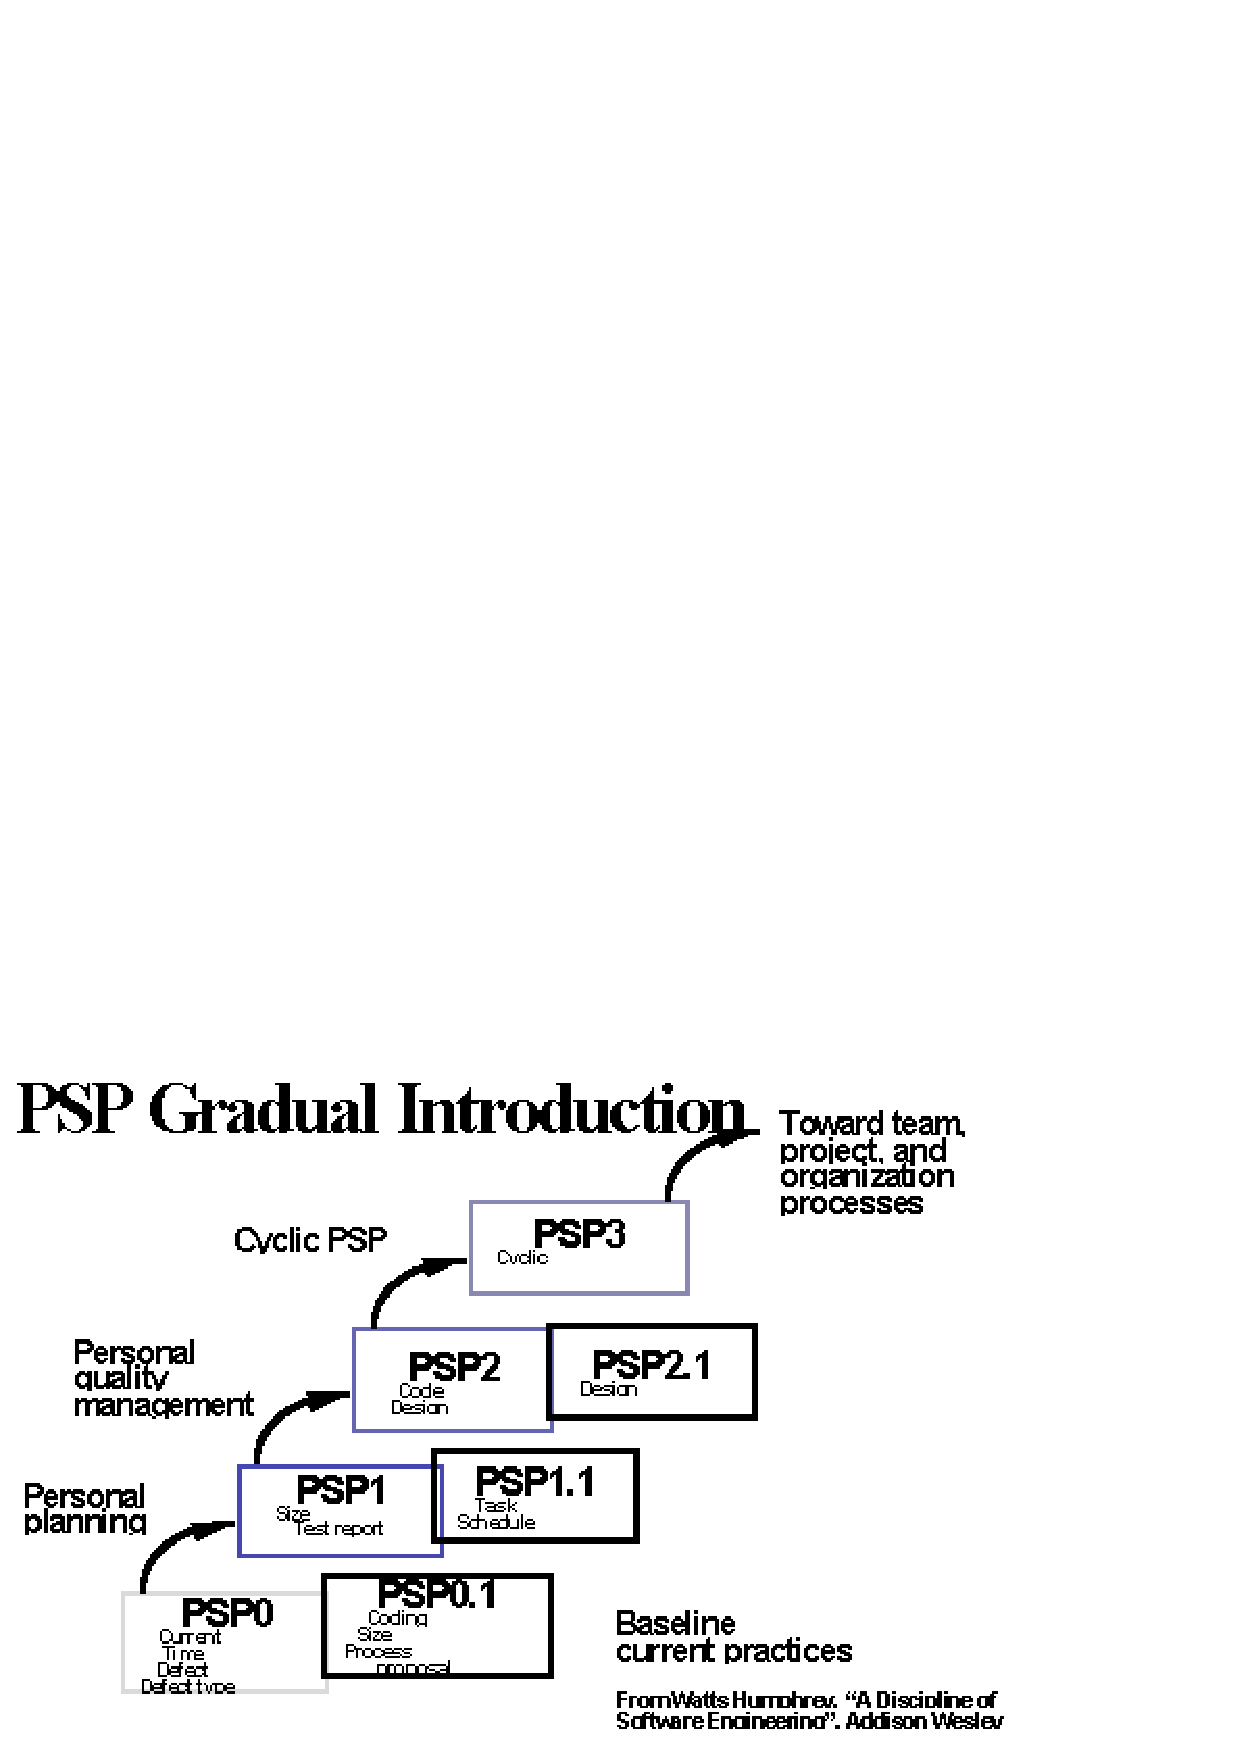
\includegraphics[height=20em]{PSP-Evo} 
   \caption{Progression of PSP}
   \label{fig:PSP-Evo}
\end{figure}

%PSP/TSP is effective in both academic education as well as industrial application. (more about related research)

Their major drawbacks are lack of automation. Developers have to manually record their process and product data (mostly the development time and number of defects). The high overhead of data collection raises a barrier to its introduction and adoption. Additionally, it is not easy to ``digest'' the data. Developers have to manually analyze their logged data in order to understand the their performance, then be able to improve it.

On the contrary, Software ICU provides a higher level of automation in tracking and analyzing software process and product data.


\section {Research Based on Automated Data Collection}
Project ClockIt and Retina are two recent research based on automated data collection to support entry-level programming courses, while PROM is the most similar research to Hackystat.

\subsection {Project ClockIt and Retina}
Project ClockIt provides a data logger as BlueJ\footnote{``BlueJ is an integrated Java environment specifically designed for introductory teaching.'' --Quoted from \url{http://www.bluej.org/about/what.html}}
 extension. It logs developer's open/close of project and package, file change and delete and compilation results. Data is logged to local file and later sent to a database via Internet. A data visualizer integrated into BlueJ is available to view data about the current project. \autoref{fig:clockit} shows an example of this visualizer. Data stored in database is used for statistic analysis such as class averages. A web interface is also available to instructors to view the individual data of their students and class average analysis data.

\begin{figure}[htbp] %  figure placement: here, top, bottom, or page
   \centering
   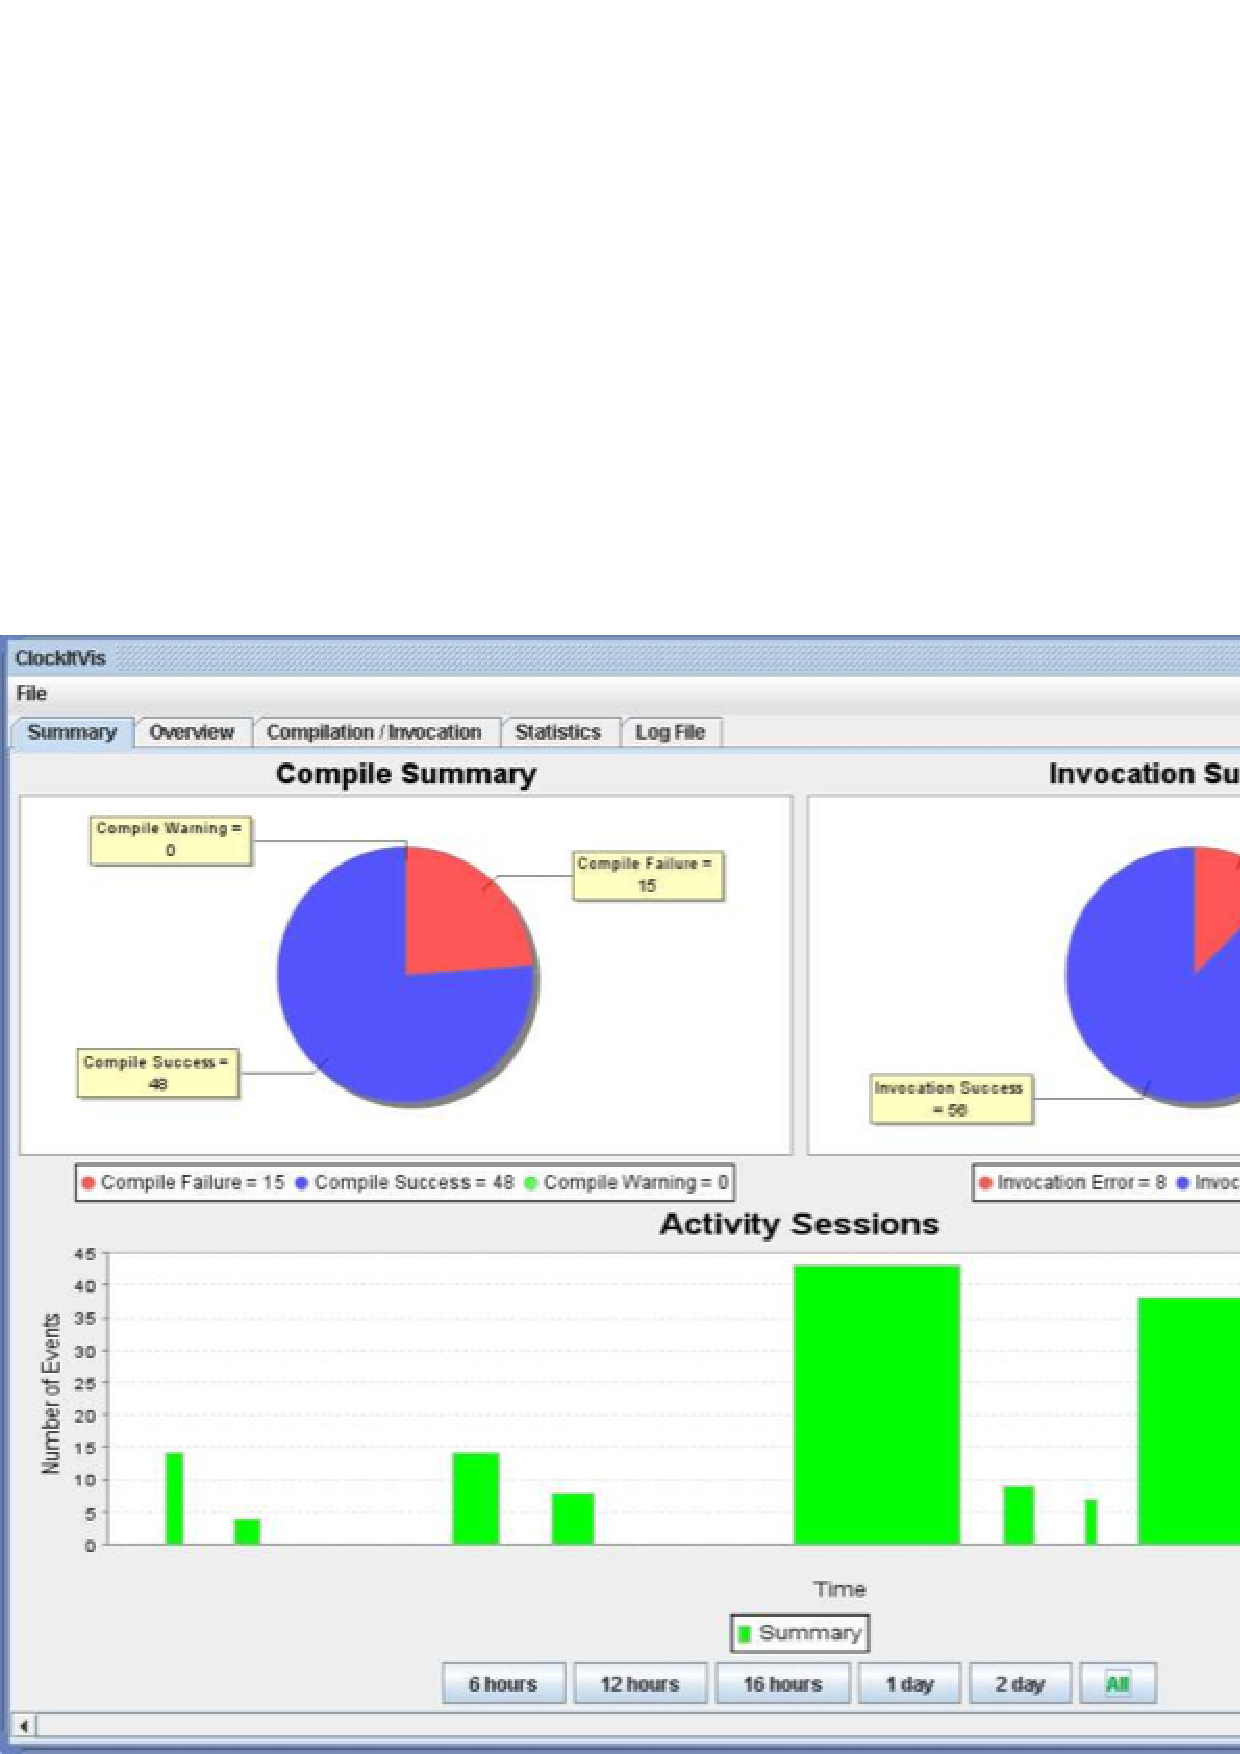
\includegraphics[height=20em]{clockit} 
   \caption{ClockIt BlueJ Data Visualizer summary}
   \label{fig:clockit}
\end{figure}

Closely related to ClockIt, Retina also provides automated data collection. Though Retina provide more tool support (BlueJ, Eclipse and command-line compiler), it focuses on a even smaller area of programming events: compilation. It gather data from students' compilation events, mostly compilation errors. In additional to its data viewer (see \autoref{fig:retina}), it also provides a recommendation tool for students. The tool use instant messaging (IM) to give students recommendation of approximated time needed for the upcoming assignment, and the compilation errors one is likely to make. These are based on both the student's previous data and the data from courses of previous semesters. 

\begin{figure}[htbp]
     \centering
     \subfigure[Retina Instructor Viewer]{
          \label{fig:retina-teacher}
          \includegraphics[width=.48\textwidth]{retina-teacher}}
     \subfigure[Retina Student Viewer]{
          \label{fig:retina-teacher}
          \includegraphics[width=.48\textwidth]{retina-student}}
          
     \caption{Data viewers of Retina.}
     \label{fig:retina}
\end{figure}

The difference between these two research and Software ICU is that they focus only on introductory level courses, where compilation is the interesting development event. In other hand, their relatively easy configuration overcomes one of the major short-coming of Hackystat and Software ICU. While neither of them provide good extensibility, they are unlikely to be useful in advanced programming situations like advanced programming course or professional setting.

\subsection {PROM}
PRO Metric (PROM) \cite{prom03} is a system that similar to Hackystat. PROM is a software system for collecting process and product metrics in a software company. It is initiated and driven by the demand of the company, and thus the research is focus on industry setting. It is designed to work fully automatically without any interaction with the user in order to get reliable and accurate data about company internal workflows and development processes. It is organized in a sequence of interconnected components, communicating using SOAP protocol. Similar to sensors in Hackystat, it has plugins for many different applications, including IDEs, word processing tools, email clients, and issue tracking systems. Data then is transit to plugin server to extract metric, then the results are sent to PROM server to store into database. \autoref{fig:promarchitecture} shows the overview of PROM's architecture.

\begin{figure}[htbp]
     \centering
     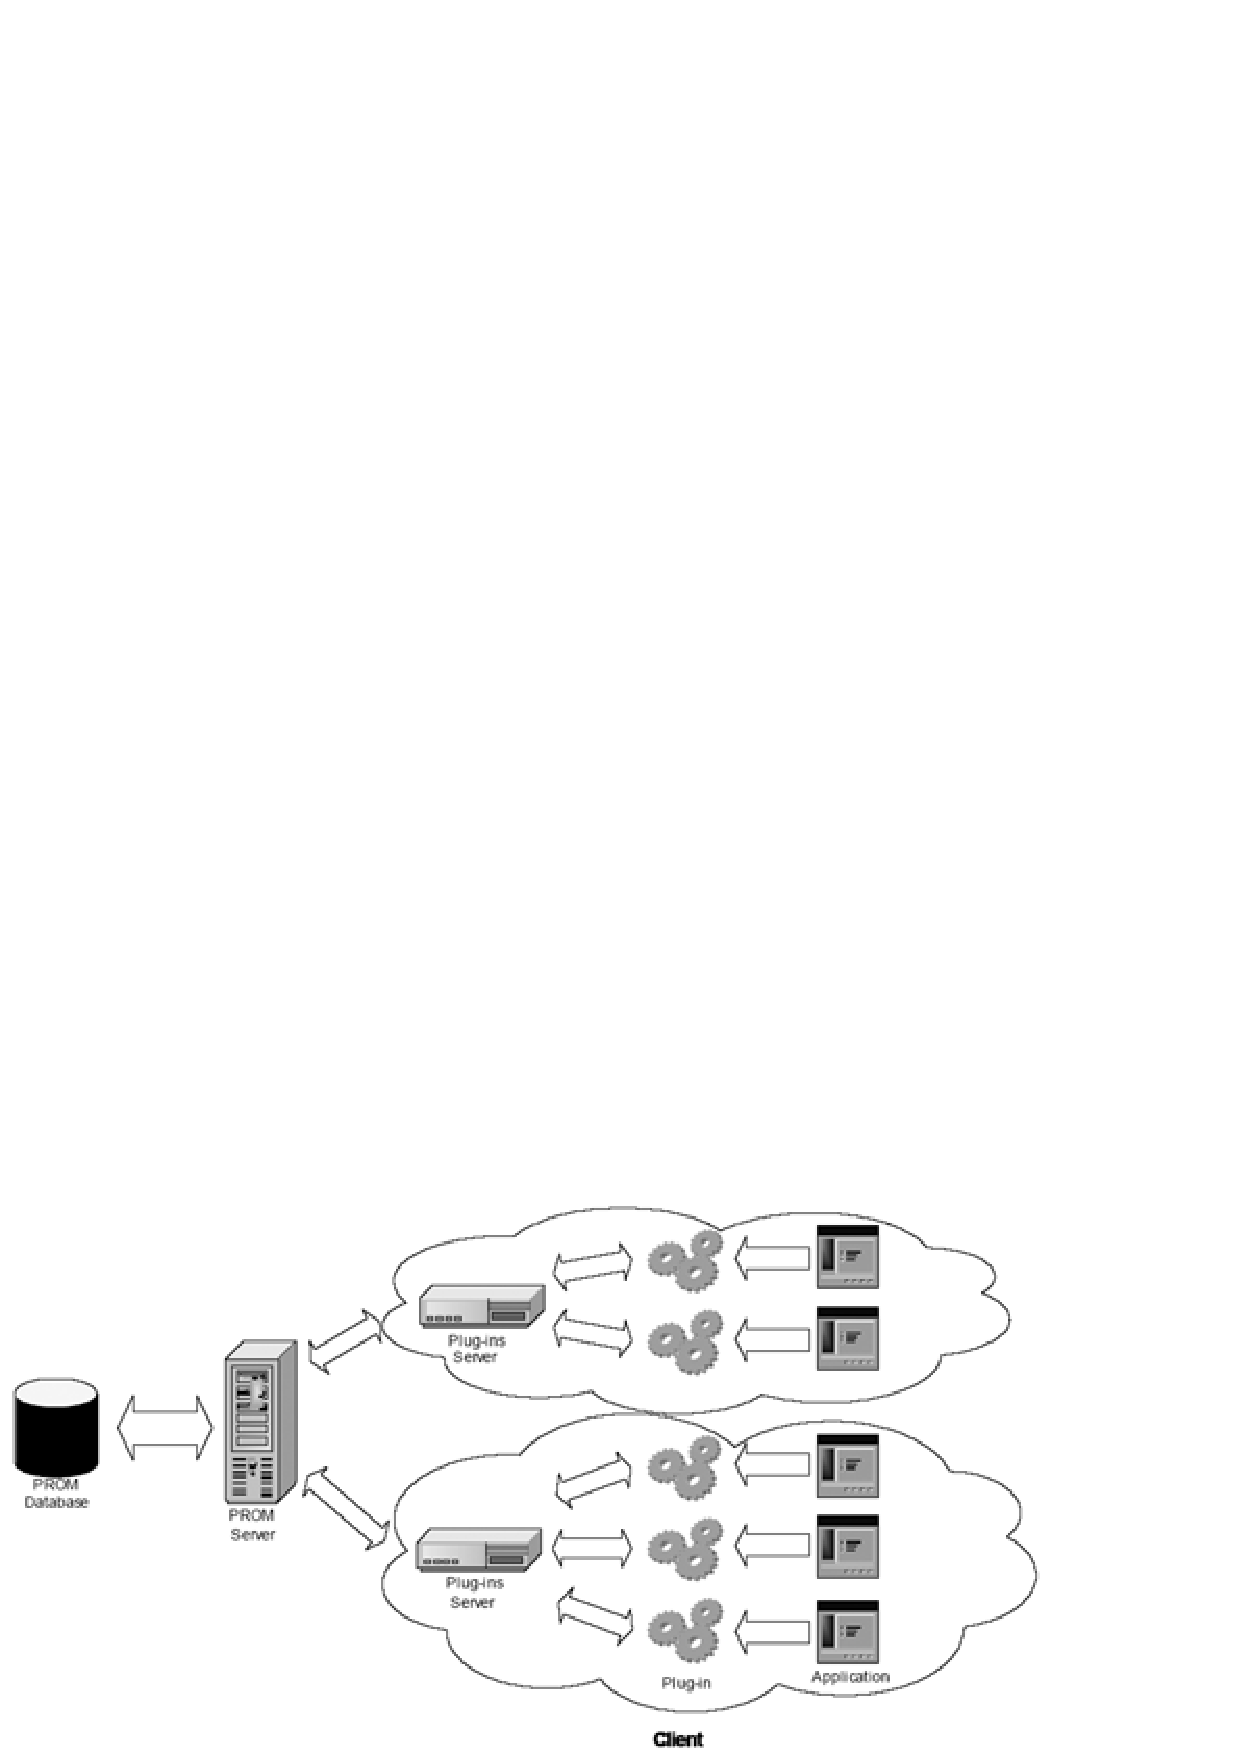
\includegraphics[width=.48\textwidth]{promarchitecture}
     \caption{Architecture of the PROM system}
     \label{fig:promarchitecture}
\end{figure}

PROM categorize users into 3 roles, developer, team leader, and manager of the team. Each of these role is provided different views of data. Developers have access to their individual, detailed data, the leader to the aggregated data of the whole team, and the manager to project level aggregated data.

Compared to Hackystat, PROM's data is stored as analyzed metrics result while Hackystat stores the raw sensor data. Different data viewers are provided to different groups of users while Hackystat provides same viewers to all users.

A case study of PROM in industrial environment\cite{prom09} discusses the lessons learn from two year experience of using the PROM system in the IT department of a large company in Italy. Evidence indicates that adopting the PROM system requires a long set-up phrase and need the company and develop team's patience and commitment to succeed, but it eventually delivers value to the company. 

One of the lessons suggest that data presentation is as important as data accuracy and simplicity, brevity and clarity is preferable. Another lesson suggest that fast aggregated view of data is desired, and users of different roles favor different aggregations, e.g. developers like reports of their daily activities, while team leader and manager like summary views of data on team and project level. Software ICU's simple and fast data presentation and high configurability and extensibility is suitable to address these requirements.

%\section {Software Project Dashboards}
%In software industry, there exists many commercial software project manage dashboards, such as LightHouse, ProjectManager.com dashboard, PivotLink Dashboards, Autotask Project Management and so forth. However, many of them are complete solution of software development business management, including not only software project states management, but also related resource allocation and budget control, etc. As being commercial products, they are not open source. Most importantly, there is few research published about these commercial project dashboards. ``Features'' are advertised as other commercial products, while short-comings are ignored. Thus negative results of their use are unknown. This research of Software ICU contains not only its benefits, but also its negative impact.


\section {Previous Case Studies of Hackystat}
The classroom study presented in this thesis is the third case study of Hackystat system in a classroom setting. 

The first case study performed in 2003 used an early version of Hackystat\cite{csdl2-03-13}. During that time, Hackystat was only collecting 4 types of metrics (Active Time, Size, Unit Tests and Coverage). The system was oriented around a set of ``Course'' analyses that were tailored to an educational setting. Those analyses summarize the individual team project metric data in tabular form, and also presented comparisons of all of the course projects\autoref{fig:hackystat2003}. The evaluation show that the installation of Ant sensors is the most significant barrier to the system. It was too difficult to install without direct help from the development team. But the overhead of use is relatively low and analyses were usable and useful. Data privacy was uncomfortable for some students.

\begin{figure}[htbp]
   \centering
   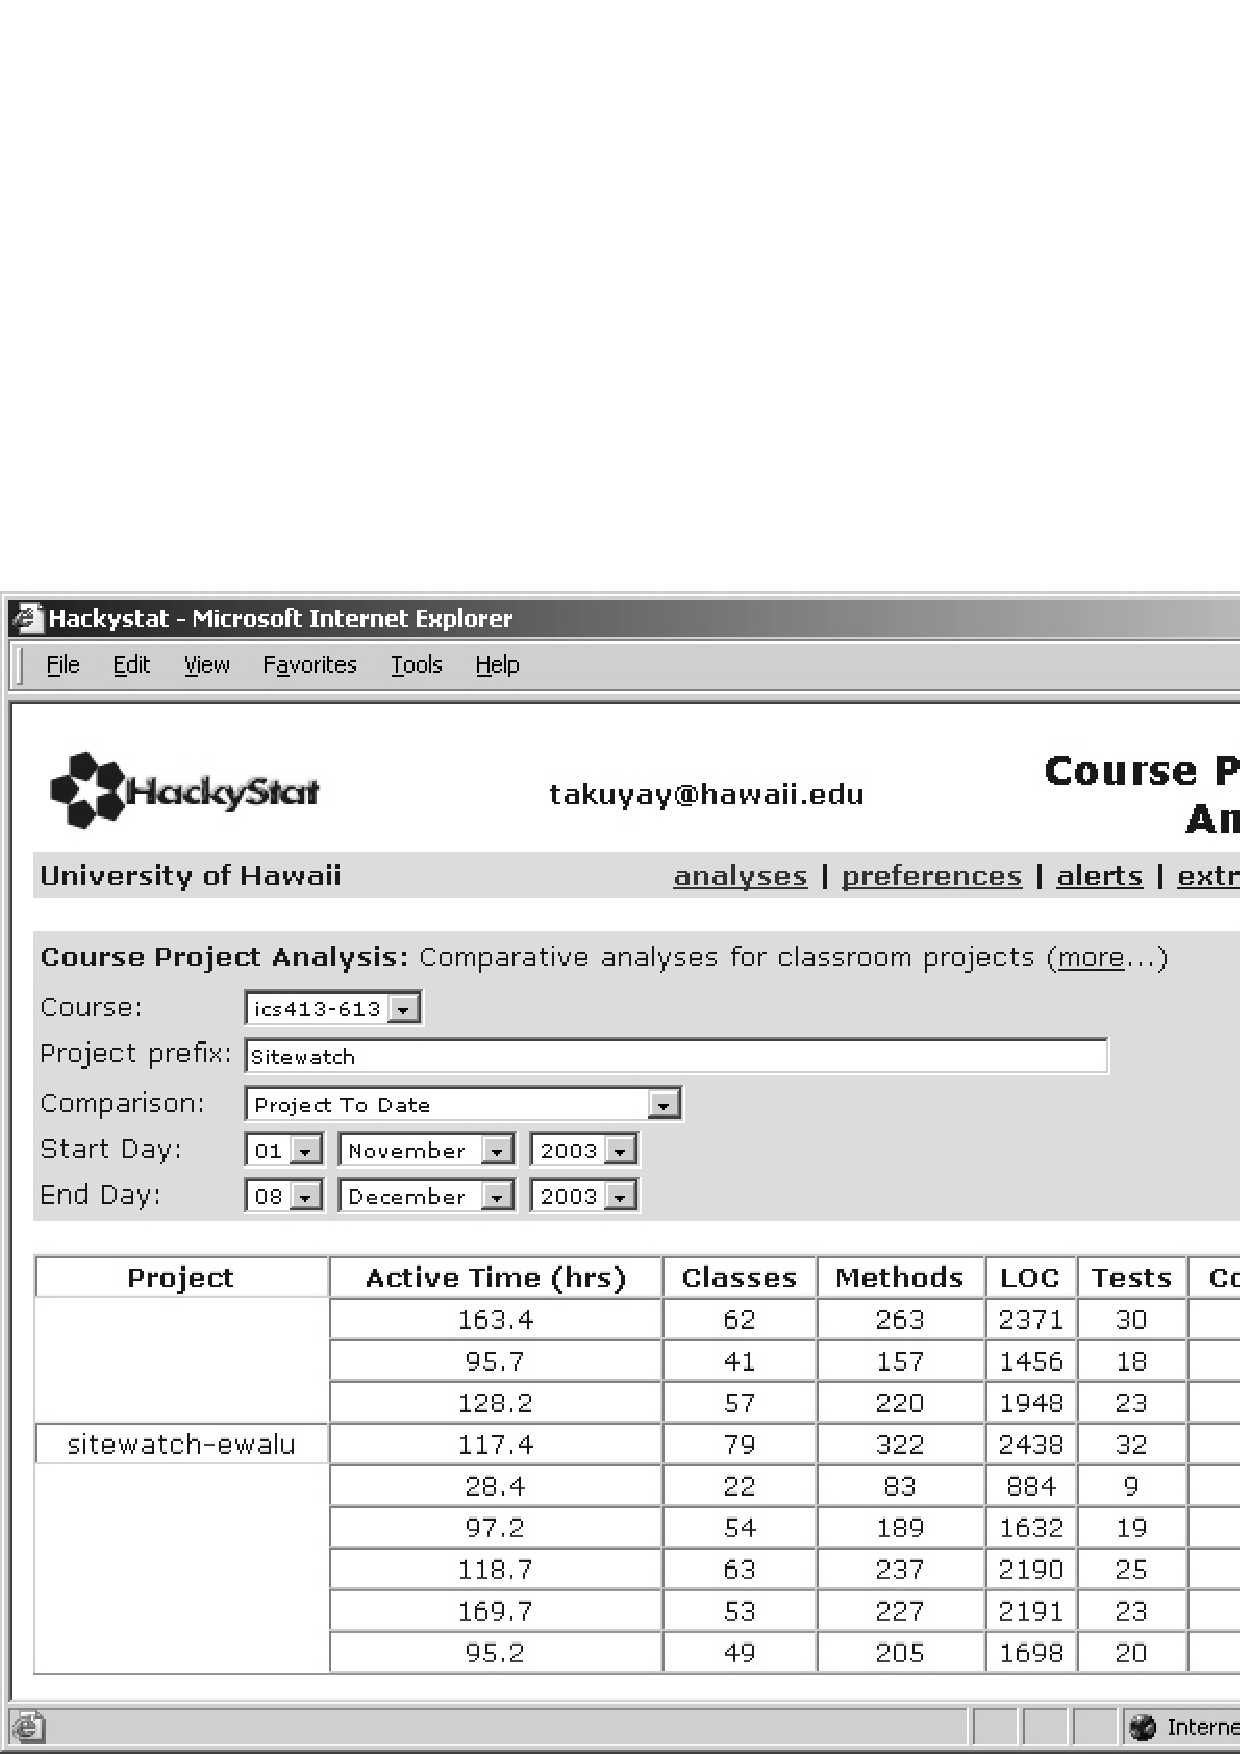
\includegraphics[height=20em]{hackystat2003} 
   \caption{Screenshot of course project to date analysis of Hackystat in 2003}
   \label{fig:hackystat2003}
\end{figure}

The second case study in 2006 is a partial replication of the first case study\cite{csdl2-07-02}. Hackystat had undergone significant change from 2003 to 2006. The sensor installation, which is the major barrier to the system in 2003, was automated by the hackyInstaller GUI, which greatly lower the overhead of configuration for developers. The evaluation also shows significant drop in sensor installation difficulty. However, new sophisticated Telemetry analysis \autoref{fig:hackystat2006} and its complex user interface raise the difficulty of using it and interpreting data, lead to slight drop in usability and professional feasibility.

\begin{figure}[htbp]
   \centering
   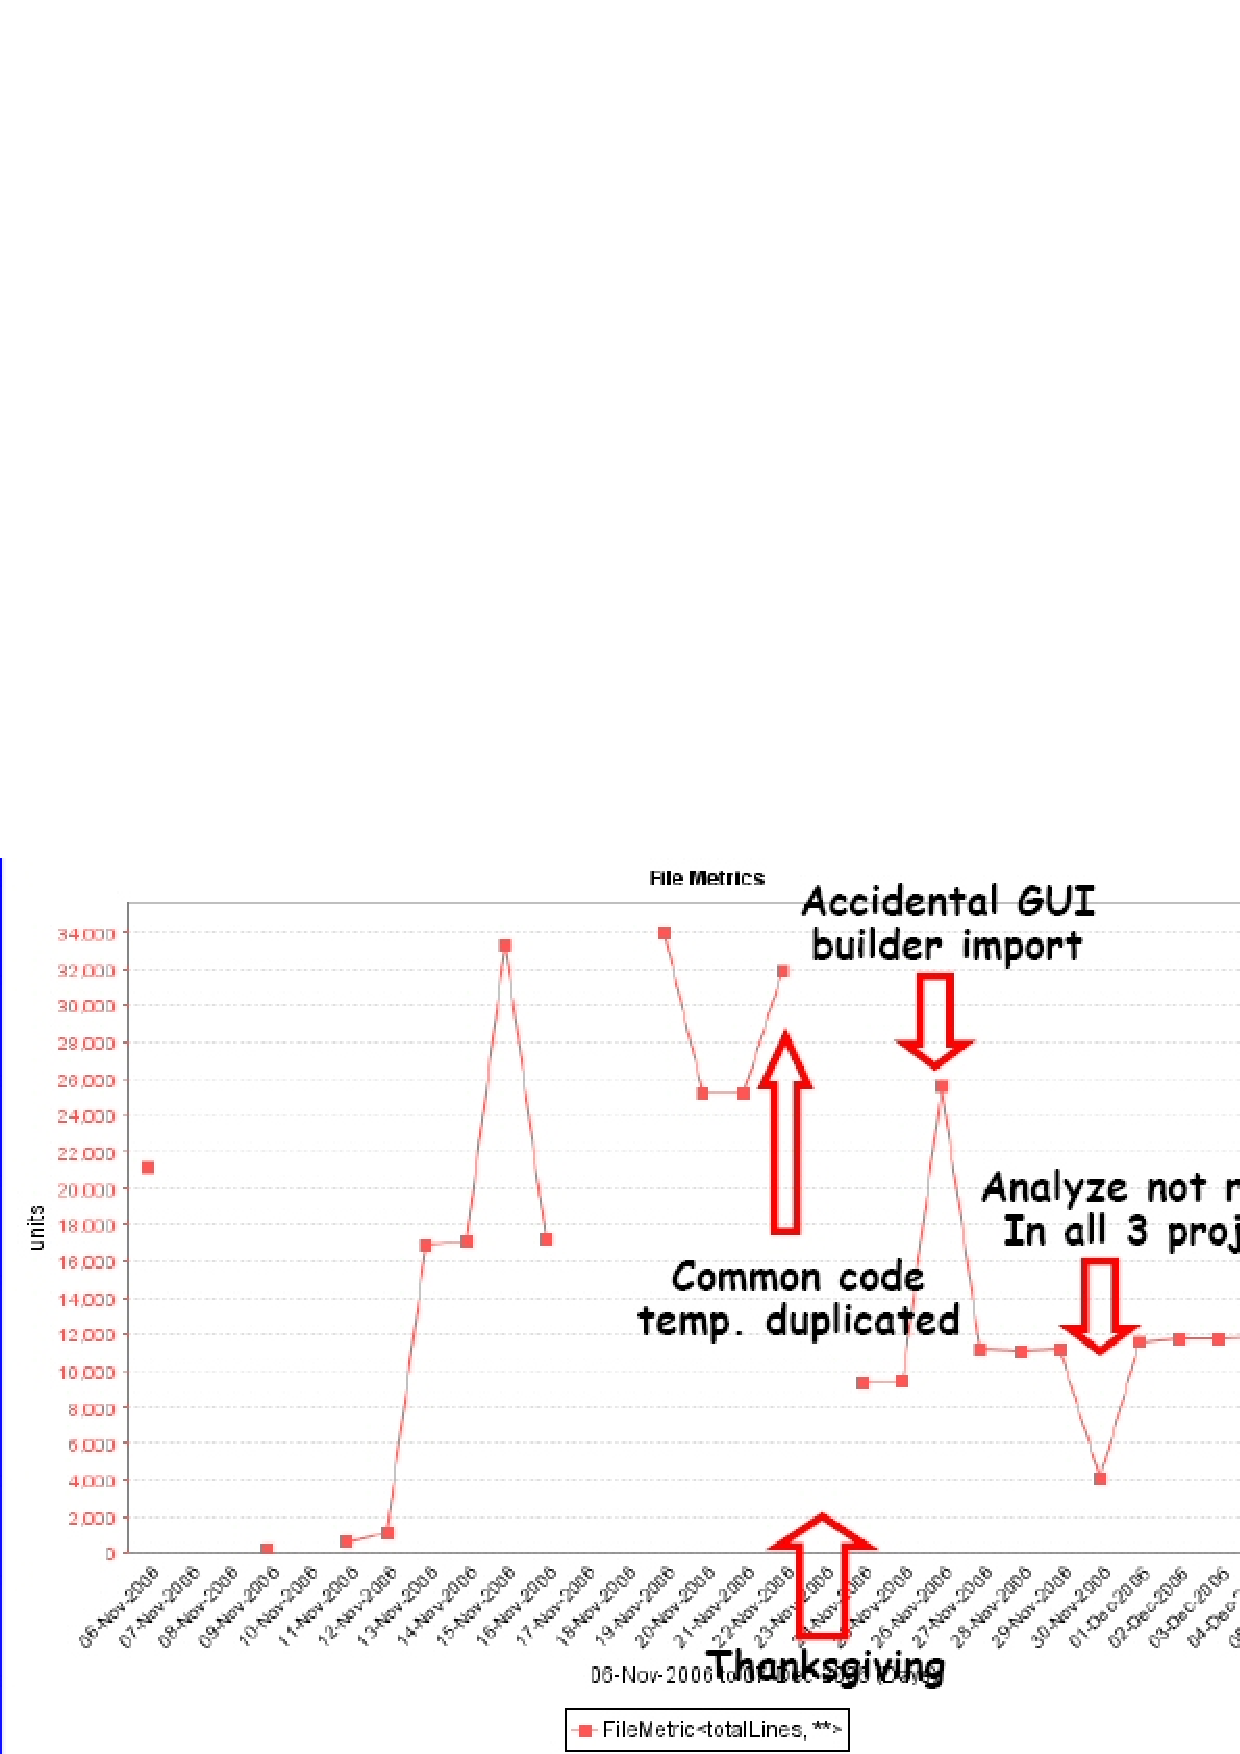
\includegraphics[height=20em]{hackystat2006} 
   \caption{Screenshot of file-metric telemetry analysis of Hackystat in 2006}
   \label{fig:hackystat2006}
\end{figure}

In 2007, Hackystat was re-implemented using a new architecture. Adopting service-oriented architecture enable  multiple user interface separate from the services components. The Software ICU is built upon a new web-based UI called Project Browser, and the classroom study is also based on this user interface.


\chapter{Hackystat}
In this research, I utilize Hackystat to implement the Software ICU. This chapter briefly introduce the Hackystat system, which was invented by Professor Philip M. Johnson, in the Collaborative Software Development Laboratory, Department of Information and Computer Sciences, University of Hawaii at Manoa. 
 
\section{Hackystat Framework}
Hackystat is an open source framework for collection, analysis, visualization, interpretation, annotation, and dissemination of software development process and product data. Hackystat consist of many software services that communicate using REST architectural principles\cite{wiki:restful}. These software services can be categorize into 4 groups, sensors, data repository, analysis services and viewers. \autoref{fig:hackystat-architecture} shows the architecture of Hackystat system. 

\begin{figure}[htbp]
   \centering
   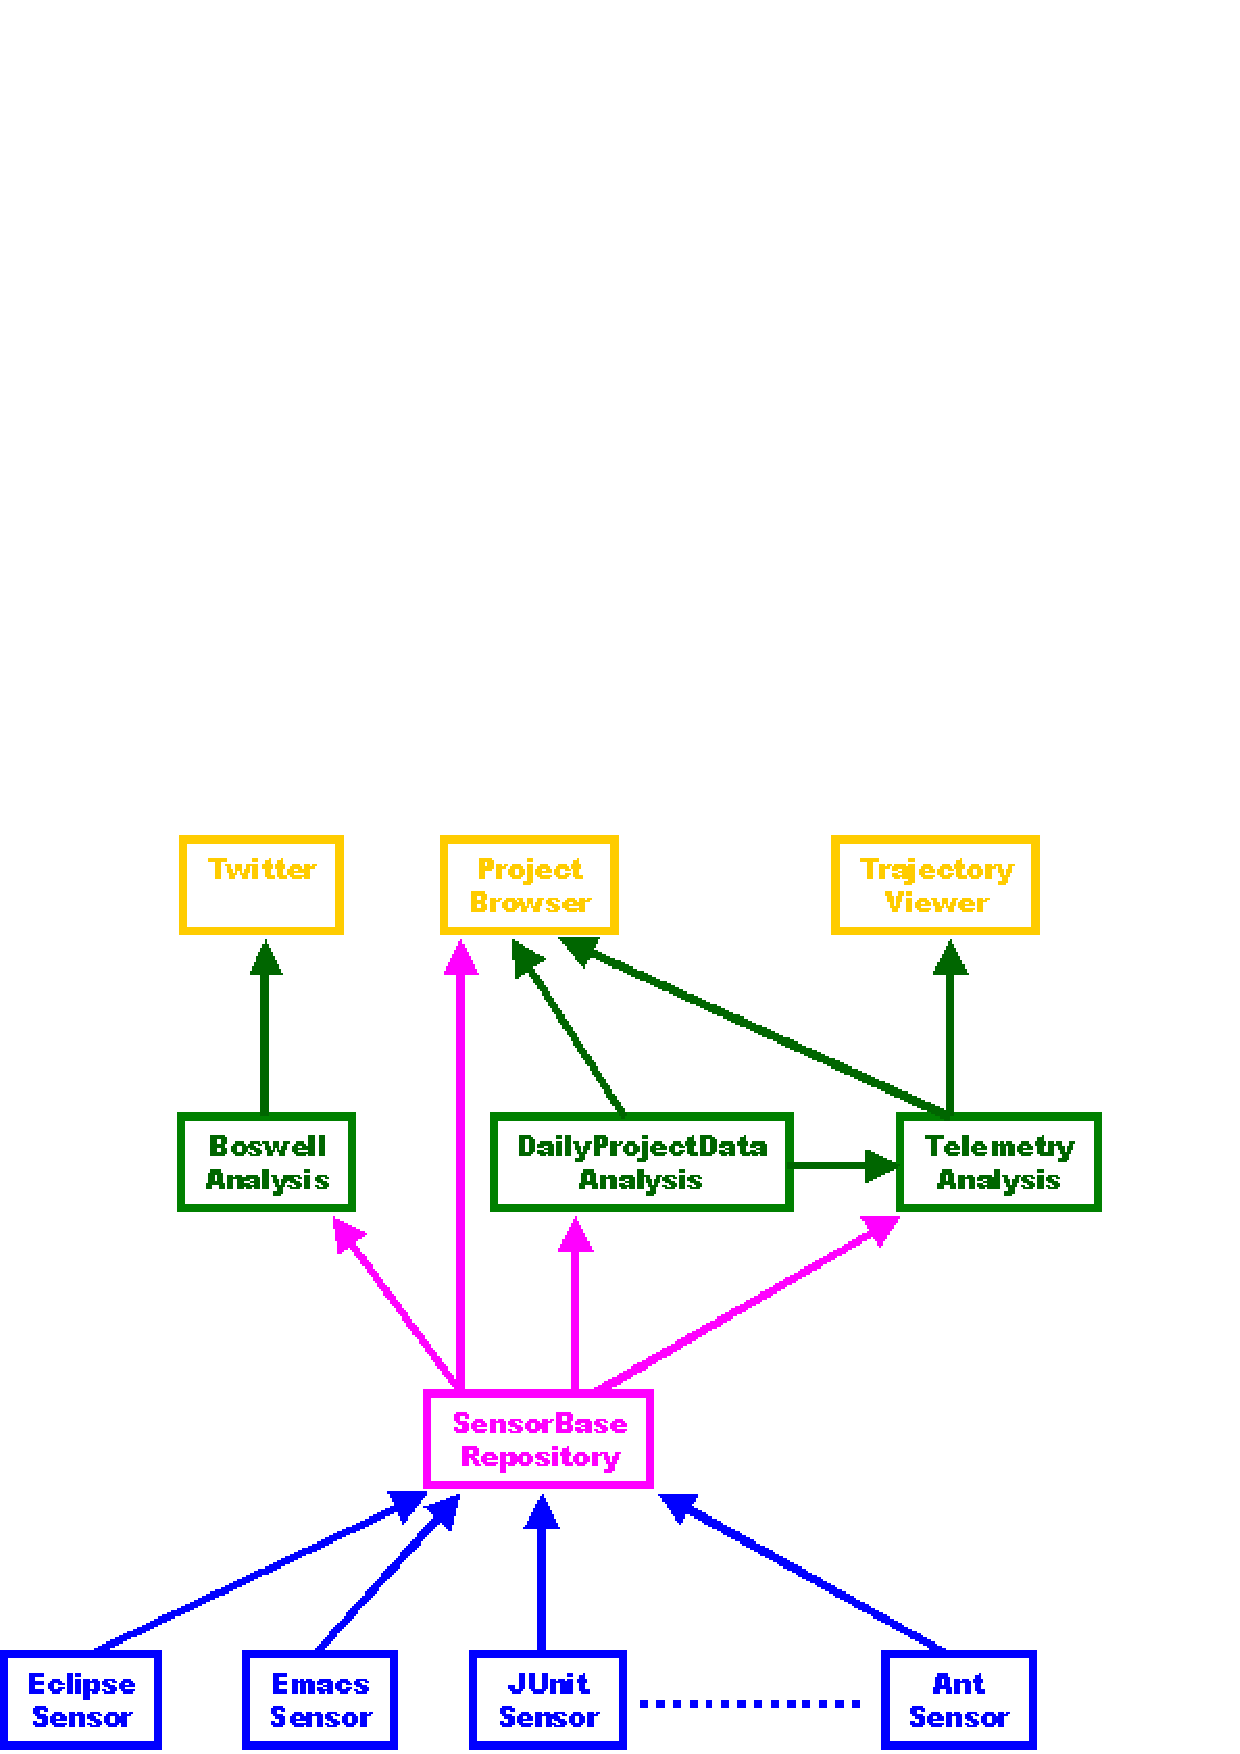
\includegraphics[height=20em]{hackystat-architecture} 
   \caption{Screenshot of file-metric telemetry analysis of Hackystat in 2006}
   \label{fig:hackystat-architecture}
\end{figure}

\subsection{Sensors}
Sensors are small software plugins that collect data from the use of tools and applications. Currently, sensors are available in many development software including Eclipse, Emacs, Ant, etc. Sensor data is represented in XML, and consist of seven basic elements: data owner, resource, timestamp, runtime, tool, Sensor Data Type and properties. The first six are required and the last one is optional. 

Sensor Data Type(SDT) is specified in every piece of sensor data when collected, so that the same type of data can be collected from different tools and higher level services can easily determine which data is relevant to them. Sensor data is designed to record only an piece of atomic data such as size of a single file, and runtime is use to group data that belongs to the same event, such as the file metric of a project. Properties are additional information for different types of sensor data, such as coverage value for coverage SDT and lines of code for file metric. 

Sensors are designed to work automatically without any attention of user besides initial configuration. In order to reduce internet communication and support offline work, data is temporarily stored, then sent to data repository every several minutes or when internet connection is available.

\subsection{SensorBase}
Sensor data is sent to the data repository, called SensorBase. SensorBase store the data as it sent from sensors, and provide RESTful interface for easy use. Sensor data can be queried with the six required elements mentioned above via HTTP calls, and data is sent back as XML. SensorBase is implemented with a database manager abstract class, thus it is easy to add support to different database implementations. Current version of Hackystat provides database support for Derby, Oracle and PostgreSQL.

\section{Analysis Services}
Analysis services of Hackystat provide abstractions of the raw data from SensorBase. DailyProjectData and Telemetry are the two most fundamental analyzes of Hackystat.

\subsection{Daily Project Data Analysis}
As its name says, DailyProjectData(DPD) service provides abstractions of sensor data associated with a single project within a 24 hour period, which represents a simple software development metric of a single day. Data of a single project includes data from all members of that project. In a DailyProjectData instance, both summary value, e.g. total development time across the project, and detail values, e.g. total development time of a project member, are available. So it is easy for higher level service to use this data.

Each DPD analysis generates software metric from data of a certain Sensor Data Type. Current available DPD analyses are Build, Code Issue, Commit, Complexity, Coupling, Coverage, Dev Time, File Metric, Issue, and Unit Test. These DPD analyses are the basic of the Hackystat system, all other analysis services are based on DPD. While DPD is the lowest level of abstraction, these can also be considered as the available software metrics in Hackystat.

\subsection{Telemetry Analysis}
Based on DPD service, Telemetry service provides abstraction over a longer period of time such as several days, weeks or months. A Telemetry Chart consists of one or more streams of data points. Each data point represents the metric value of in a single granularity (day, week or month). Together they show the trend of the metric(s).

There is a special group of Telemetry charts called Member-Level Telemetry. These charts consist of several stream, each of which belongs to a project member. They are used in Software ICU's drill down feature to compare performance of each member within a project. 

To support the work practices of different organizations, Telemetry service provides a domain specific language that allows to build new Telemetry Chart with Telemetry stream lines. The predefined Telemetry Charts are all written with this language.

Telemetry streams can also accept parameters to refine the object data. This feature is inherited in Software ICU, where user can configure the parameters of each Telemetry analysis of each vital sign (more detail discuss in \autoref{vitalSign} and \autoref{SICUconfiguration}).

\section {Project Browser}
Project Browser is one of the viewers in Hackystat system. It is based on Wicket\footnote{\url{http://wicket.apache.org/}}, a Java-based web application framework. Project Browser is integrated with viewers to all Hackystat services, which are organized as tabs. 

With help of Wicket's modularization, viewers on Project Browser can share many common panel, such as project/date selection panel and Ajax loading process panel, which facilitate the development of new page. This also makes user's experience more consistent across different viewers. Therefore it now serves as a data presentation and high level analysis development center. Several new presentations and high level analysis are developed upon it, Software ICU is one them.

\chapter{Design and Implementation of Software ICU}
In order to achieve good governance of software development projects, we adopt the metaphor from medical ICU and develop a system called Software Intensive Care Unit. It consists of a set of vital signs, each of which is based on one software development metric and indicates the project's ``health'' state from one perspective.

Interface of Software ICU is separated into two part. The left-hand side is the control panel, where user can pick the analysis period, data granularity and select projects to analyze. The right-hand side consists of three panels: the data panel, the loading process panel, and the configuration panel. Each of these panels is discussed in following sections. Data panel is the major panel to show the result of SICU analysis. \autoref{fig:overview} shows an example of Software ICU.

\begin{figure}[htbp]
   \centering
   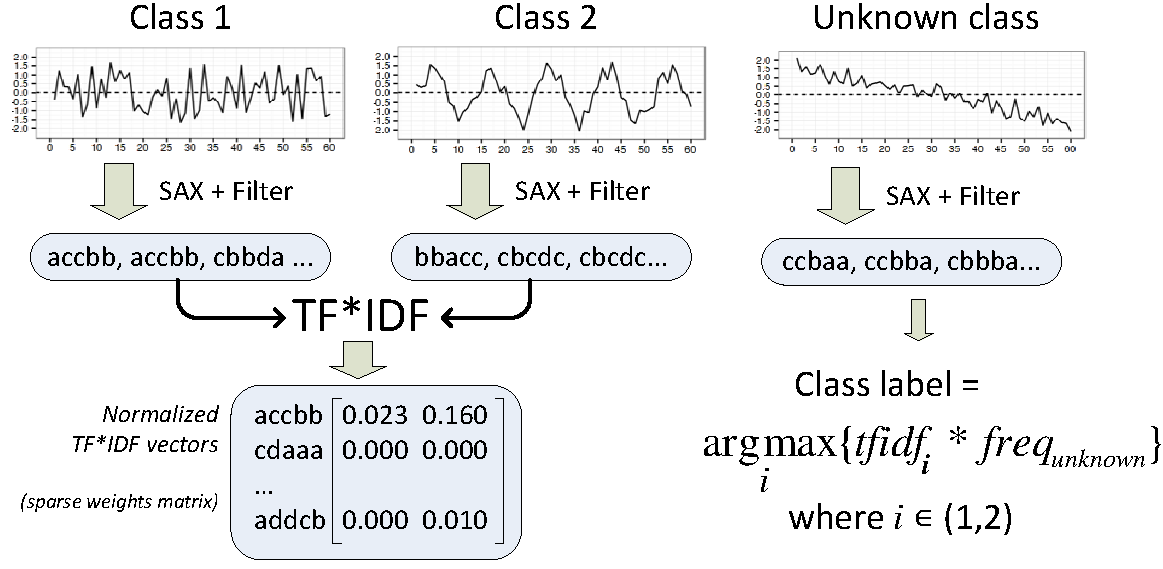
\includegraphics[width=\textwidth]{overview}
   \caption{A screenshot of Software ICU}
   \label{fig:overview}
\end{figure}

\section{Vital Signs}
\label{vitalSign}

Similar to medical ICU, using multiple software development metrics in Software ICU are necessary because there is not a single metric can determine the health state of a software project. Similar to medical vital signs, each software metric show the process or product state from different aspect. And changes in one of them may or may not indicate a change in health state, but changes in more of them indicates higher possibility that health state changed. In this study, we use nine vital signs in Software ICU.

Vital signs of software projects are measured by various software development process or product metrics. Each of these vital sign reveal an aspect of the health state of the software project. In this section I will discuss all these vital signs.
\begin{description}
\item[Coverage] 
Coverage is a good indicator of the tests' quality. It stands for the test coverage of source code in unit testing, which usually measured as the percentage of code units (line, method, class, etc) that is executed during unit test. There are a number of coverage criteria, such as line, method, class, conditional, etc. In Software ICU, user can select which to use. No matter which criteria to use, higher coverage is always better because higher percentage of code covered by unit testing indicates lower risk of existence of bug in untested code segment. However, high coverage does not necessary mean good quality of unit test, and vice versa. One of the reason is that, in some situations, it is difficult to achieve high test coverage because of the difficulty of verifying results, especially when using UI frameworks. Another reason is that the code executed during unit testing can be unverified. For example, when testing an image processor with a given image file, the code of loading the image file is executed, but the test does probably not have assertion about the correctness of loading the file. But as long as developers don't have the intend to trick coverage in order to pretend to be writing enough unit tests (It is possible if coverage is used to judge their performance.), raising coverage is always a good thing.

\item[Cyclomatic complexity] 
Cyclomatic complexity, a measurement of the complexity of a program developed by Thomas J. McCabe, measures the number of linearly independent paths through a program's source code\cite{mccabe:complexity}. The higher cyclomatic complexity, the more distinct control paths in a program module, and the more difficult to achieve high path test coverage. Additionally, code of high complexity is difficult to understand, thus it is hard to maintain. Therefore, program modules are preferred to have lower complexity. But high complexity is not necessary evil. The nature of some programs just require high level of complexity. Also raising in complexity is sometimes unavoidable during development, especially when optimizing code performance. However, developers should try to lower complexity, especially in early stage of development, so that it is easier for future maintenance.

\item[Coupling] 
Coupling, or dependency, is the degree to which each program module relies on each one of the other modules\cite{wiki:coupling}. It is a measurement of the complexity of the whole system's module reference tree. Whenever one module is modified, there will be a chance that the changes may cause bugs in one of modules that relies on it. Therefore, higher coupling implies higher risk of introducing bugs when making changes, thus harder to maintain. High coupling might also be harder to reuse because dependent modules must be included. Therefore, Coupling is suggested to be kept low.

\item[DevTime] 
DevTime, abbreviation of Develop Time, is a measurement of develop time of developers. Hackystat use a special approach to measure this: for each 5 minutes interval, if there is anything development activities happen, the developer is consider developing in that interval. It relax the criteria of measuring develop time so that coding while reading from documentation will get the same DevTime as intensive coding period. Thus it is more accurate than previous ActiveTime in older Hackystat. However, Hackystat sensors for DevTime are only available in several IDEs (currently available to Emacs, Eclipse, and Visual Studio). No sensors are available for other applications that might be used during developing, such as browsers, E-mail clients, office systems, or other editors/readers. So the monitored development activities is limited. Moreover, some developing activities, such as reading and learning, are very difficult to track. Therefore, DevTime should not be simply used to determine a developer's effort. But as habit of an individual will not change a lot, so the DevTime of a developer should be relatively stable over time. Thus large sudden increase in DevTime is a possible sign of bad developing habit like ``start late near deadline''.

\item[Churn] 
Churn is a measurement of the change (add, delete and/or modified) of code that is made into repository. It is usually measured by LOC (lines of code). It is an indicator of developers' contribution to the project. Interpretation of this metric is conditional. In the early stage of development, churn is expected to be higher because new codes are keep being added. During the maintenance of a system, churn is mainly from fixing bugs and adding new features, both of which are fewer for a stable system, thus churn is expected to be lower. In terms of develop behavior, churn of a developer reflects the amount of work of him/her. It tends to be relatively stable over time in the same project because the work rate of an individual does not vary a lot in the same coding condition. Dramatically change in churn of an individual developer while DevTime not changing respectively is a bad phenomena, which might due to bad developing habit like ``copy and paste without understanding''.

\item[Commit] 
Commit measure the number of commitments made into repository. ``Commit early, commit often'' is one of the well-accepted guideline of continuous integration. For the same amount of churn, more commits implies better following of this discipline.

\item[Size] 
The size of the project is measured by the source lines of code (SLOC), which counts the number of lines in the text of the program's source code. It can be a sign of the effort put into the project, However, SLOC alone does not make as much sense about the state of the project as Churn. We include this vital sign only to give user an idea of the size of the project, just like the height in your medical record.

\item[Test] 
Test is a count of unit test tasks invoked in a period of time. Unit testing is a software verification and validation method in which a developer tests an individual units of source code. It is used to ensure that code meets its design and behaves as intended. A requirement of good development behavior is to test while coding, or event better, use ``Test Driven Development'' (TDD). No matter what development pattern to follow, unit testing is a dispensable component and regular execution of unit tests is always a good sign of ``health'' development habit.

\item[Build] 
Build is a count of ant build task invoked in a period of time. A build task accomplish all necessary step to ensure the correctness of the code before commit. It consists of compilation, code inspection, unit testing, documentation generation, etc. It is an usual activity in software development nowadays. Though how often to build largely depends on personal preference and habit, it is advised to build often to ensure the correctness of the system.

\end{description}

These nine vital signs are the default set in Software ICU, but not the only setting. Users can determine to use which vital signs in their setting, as well as creating new vital sign analysis with Telemetry charts. More detail about these configuration and customization are discuss in \autoref{SICUconfiguration} and \autoref{SystemCustomization}.

\section{Vital Sign Presentation}
\label{presentation}
As reported in case study of PROM, data presentation is as important as data accuracy\cite{prom09}. One of our primary goal of Software ICU is to provide a proper presentation to help interpret large amount of software metrics data. In order to achieve this goal, Software ICU use mini charts to integrate historical data and use color to categorize the health state of a vital sign.

A vital sign analysis consists of two part: a numerical latest value and a mini historical chart. 
\begin{description}
\item[Latest Value] represents the newest state of the vital sign in the analysis period. In our implementation, it shows the most recent associated DailyProjectData. If there is no DPD on the latest date of the analysis period, it will search back the time period for the first available data of that DPD. The latest value will be ``N/A'' only when there is no any data of that metric in the whole analysis period.
\item[Mini chart] represents the trend line of the associated metric data over the analysis period. This mini chart is implemented as bar charts. Each bar represents the DailyProjectData value of the metric on a unit of granularity (day, week or month). Bars heights are scaled so that the highest bar is almost reach the top of the chart.
\end{description}

However, only use the last values and mini charts does not address the requirement of fast data interpretation. Thus we further enhance the representation by adding colors to those numerical values and charts to provide intuitive idea of the ``health'' state of the vital signs.

Generally, we use color green to represent ``healthy'' state, red to ``unhealthy'' state, and ``yellow'' to state between green and red or uncertain. This is color pattern is good for indicating states because it match the convention people comprehend color and thus most people can understand it without reading instructions.

Different vital sign may use different coloring method, and the latest value and the mini bar are colored separately. Choice of coloring method mainly depends on the nature of the vital sign. In general, vital signs that have clear preference of higher or lower, like most based on software development product metrics (Coverage, Complexity, Coupling) will use Stream Trend Coloring method, and vital signs based on software process metrics will likely to use Participation Coloring method. Sometimes, there may be no ideal coloring method for a vital sign, such as FileMetric, then user can select to leave that vital sign uncolored.

\subsection{Stream Trend Coloring} 
Stream Trend Coloring method determines the health of a metric by its value and trend. It colors the latest value as well as the mini chart. It takes three parameters: {\it HigherBetter}, {\it Higher Threshold} and {\it Lower Threshold}. User can decide the preferable trend, higher or lower, using the {\it HigherBetter} parameter. A raising mini chart is considered to be good/bad if the {\it HigherBetter} parameter is set to true/false. A trend is considered to be raising if there is no any value point is lower than the one before, and the last value is greater than the first value. Falling trend is considered the same opposite way. In order to be able to categorize trends that have some small disruption as raising or falling, the Stream Trend Coloring method consider small amount (proportionate to the average of the first and the last value) of change as equal. Stable trends are always considered as ``healthy'' because in that case it is as good as ``healthy'' that user doesn't need to pay much attention to it, while the actual value will be shown in the latest value where the value will be judged to be ``healthy'' or not. And unstable trend is marked as yellow because it is no fast way to tell if it indicates a good state or not. 

{\it Higher Threshold} and {\it Lower Threshold} parameters are only used when coloring the latest value. Values exceeds the higher threshold will be colored green if {\it HigherBetter} is true, or red if {\it HigherBetter} is false. Values lower than the lower threshold are colored in similar way. Values between these two thresholds are always colored yellow.

\subsection{Participation Coloring}
Participation Coloring method determines the health of a stream by the participations of all members in the project. It only colors the mini chart, leaving the latest value uncolored. This coloring method is designed to detect the health state of team cooperation, mainly via software process metrics. It takes three parameters: {\it Member Percentage}, {\it Threshold} and {\it Frequency}. Participation Coloring method colors a mini chart green if 
\begin{enumerate}
\item there are more percentage of members than the {\it Member Percentage} parameter that,
\item have the metric value greater than or equal to the {\it Threshold} parameter per day,
\item for more frequently than the {\it Frequency} parameter in the analysis period.
\end{enumerate}

A mini chart is colored yellow if it does not meet the green requirement, but the metric of the team as a whole meet the requirement of green, i.e., 
\begin{enumerate}
\item the combined metric value is greater than or equal to the {\it Threshold} parameter per day,
\item for more frequently than the {\it Frequency} parameter in the analysis period.
\end{enumerate}

If the yellow requirement is not meet neither, the mini chart will be colored red.

In other words, Participation Coloring method color a vital sign green if most members of a project are making noticeable contribution to the project regularly, and color it yellow if not but there is someone making contribution to the project in most of the time, and color it red otherwise, which means, in terms of this vital sign metric, the contribution of members to the project is rare and/or insignificant.

\section{Mini Chart Drill-Down}
In each non-empty mini chart, Software ICU provides a link of the drill-down Telemetry analysis. The drill-down Telemetry analysis is the analysis that used to generate the mini chart. For most of software product metrics, such as Coverage, Complexity and Coupling, the drill-down Telemetry analysis will show the same chart as the mini chart in Software ICU's vital sign block, just in different style with more detailed axes. However, for software process metrics, instead of the original chart, an associated member-level Telemetry analysis is shown when drill-down. 

The member-level Telemetry shows multiple stream lines in the chart, each of which represents the analysis of a member of the project. From this member-level Telemetry, it is easy to see members' participation to the project in this metric. This is most useful when combined with the Participation Coloring in Software ICU, where you see the summary result of members' participation, and then understand the detail with member-level Telemetry analysis.

The drill-down Telemetry analysis use the same parameters as used in Software ICU, thus the non-member-level chart should be identical with the one in Software ICU. Vital signs with drill-down to member-level Telemetry, use as well the member-level Telemetry to generate the mini chart in vital sign block by summing all stream lines into one. Software ICU provides different integrating method to handle vital signs that use member-level Telemetry, more detail is discussed in \autoref{SystemCustomization}.

\section{Vital Sign Configuration}
\label{SICUconfiguration}
Software ICU provides user full access to the configuration of each vital sign. User can enable/disable a vital sign, choose its coloring method, and configure the parameters of the associated Telemetry analysis. 

\begin{figure}[htbp]
   \centering
   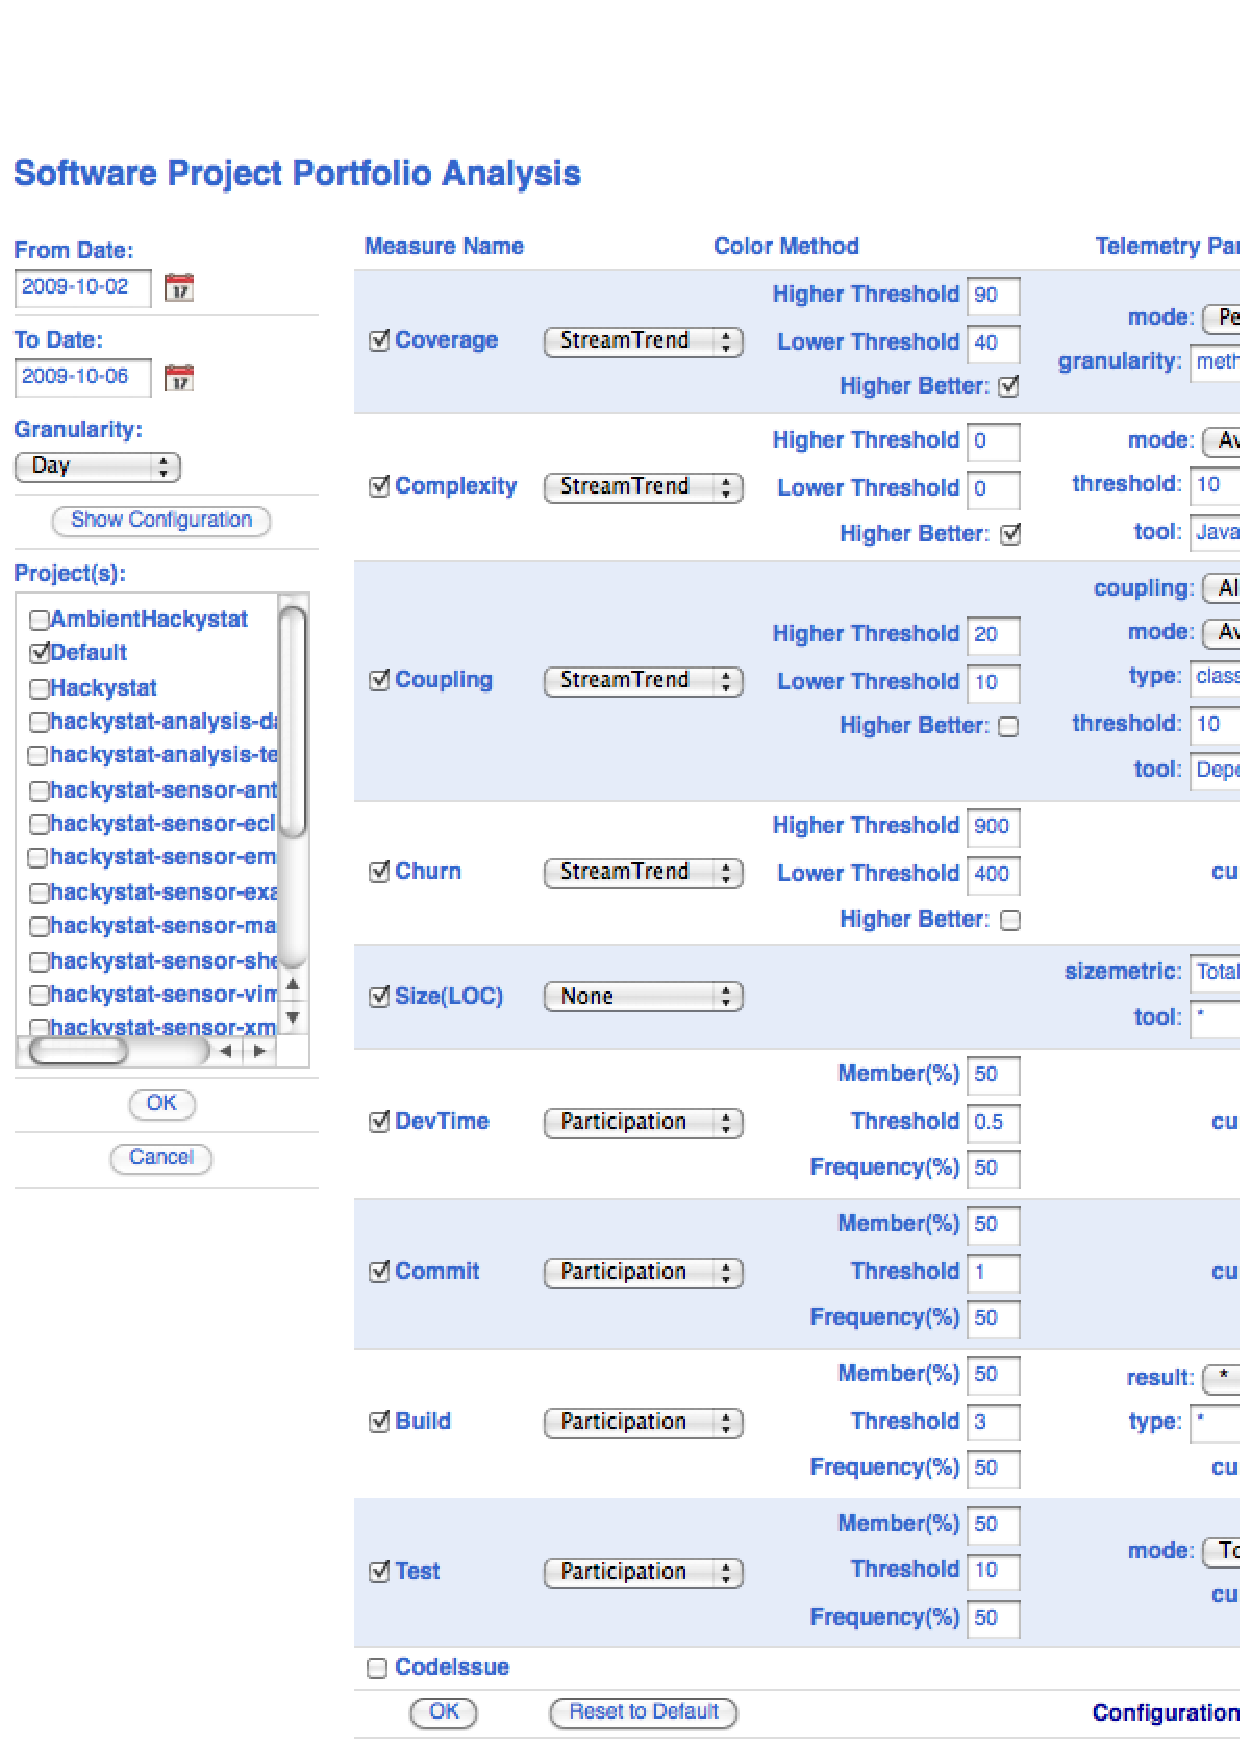
\includegraphics[width=\textwidth]{SICU-configuration} 
   \caption{The Vital Sign Configuration panel in Software ICU}
   \label{fig:SICU-configuration}
\end{figure}

By clicking the ``Show Configuration'' button in the input panel on the left, user can open the configuration panel to its right. Then the ``Show Configuration'' will be disabled when the configuration panel is shown. \autoref{fig:SICU-configuration} shows an example of the vital sign configurations. The first column is the name of the vital sign with the checkbox to enable or disable a vital sign. When a vital sign is disabled, the configuration of color method and Telemetry parameters will be disappear, however, the settings are not discarded, thus when enabled again, it be the same before disabled. The second column is the color method. Current version of Software ICU provide three choices: StreamTrend, Participation and None. By choosing the first two, its associated parameters, which discussed in \autoref{presentation}, are shown next to the drop-down selection field. When ``None'' is selected, nothing will be shown in that space. The last column is the Telemetry parameters, which is defined in the definition of Telemetry charts, and will be directly transferred to Telemetry service when retrieving Telemetry analysis for vital sign presentation. Because of the implementation reason, results of enabling/disabling a vital sign and selecting different color method will be saved immediately, but other fields will only be saved when the ``OK'' button in the bottom is pushed. When the ``OK'' button is pushed, the configuration panel will disappear after setting is saved, and the ``Show Configuration'' button will become available again.

In order to persist user's configuration setting between each visit, the configuration settings are saved in server side using UriCache. UriCache is a wrapper around the Apache JCS system\footnote{``JCS is a distributed caching system written in java. It is intended to speed up applications by providing a means to manage cached data of various dynamic natures.'' --\url{http://jakarta.apache.org/jcs/}}. It is designed to provide an API well suited to the needs of Hackystat services. The vital sign configuration objects are directly cached, under the name of the user. The cache expiration timer is set to 300 days so that it will not easily be expired. But if the cache is expired, the system will use the default setting of the vital signs.

Next to the ``OK'' button is the ``Rest to Default'' button. It will restore all vital sign configuration settings to default, and the result of restoring will be shown and saved immediately. 

In the bottom-right of the configuration panel is a link called ``Configuration Instructions''. When clicked, it will show a simple instruction of the configuration panel in a pop-up window.


\section{System Customization}
\label{SystemCustomization}

Beside the ability to configure vital signs on the fly, Software ICU provide also offline customization of default vital signs. All vital signs, including the default set discussed above, are defined in PortfolioDefinition XML files. There are two place the system will look for these XML files. The first place is inside the package of detail panel of Software ICU, where the default set of vital signs are defined. The other place is ~/.hackystat/projectbrowser/, where ``~'' stands for user's home directory. Here is an example of the definition XML file:

\begin{verbatim}
<?xml version="1.0" encoding="utf-8"?>
<PortfolioDefinitions>
  <Measures>
    <Measure name="Coverage" 
             classifierMethod="StreamTrend" 
             enabled="true"
             telemetryParameters="Percentage,method">
         <StreamTrendParameters higherBetter="true" 
                                lowerThresold="40" 
                                higherThresold="90"/>
    </Measure>
    <Measure name="MemberDevTime" 
             alias="DevTime" 
             merge="sum" 
             classifierMethod="Participation" 
             enabled="true">
          <ParticipationParameters memberPercentage="50" 
                                   thresoldValue="0.5" 
                                   frequencyPercentage="50"/>
    </Measure>
    <Measure name="FileMetric" 
             alias="Size(LOC)" 
             enabled="true">
    </Measure>
  </Measures>
</PortfolioDefinitions>
\end{verbatim}

There is a root element called {\it PortoflioDefinitions}, enclosing a single element {\it Measures}. Within the {\it Measures} element, there are a set of {\it Measure} element, each of which stands for a vital sign. Each {\it Measure} element can take up to six attributes:
\begin{enumerate}
\item The {\it name} attribute is required. It is the name of the Telemetry analysis used in this vital sign.
\item The {\it alias} attribute is optional. When it is set, it will be used as the name of this vital sign. Otherwise, the {\it name} attribute will be used as this vital sign's name.
\item The {\it classifierMethod} attribute defines the default coloring method, either StreamTrend or Participation. This attribute is optional. When it is unset, the default coloring method will be none.
\item The {\it enabled} attribute defines if the vital sign is enabled by default. If set to false, the vital sign will be disable by default. But user is still able to enable it in configuration panel.
\item The {\it merge} attribute defines the method to integrate multi-stream telemetry. It is necessary for member-level telemetries to work. ``sum'', ``min'' and ``max'' are available choices. If it is unset, the first stream of the telemetry will be used. Because of the order of streams in a multi-stream telemetry is not guaranteed, use member-level telemetry without setting this attribute might cause unexpected result.
\item The {\it telemetryParameters} attribute is the Telemetry parameters of the telemetry analysis defined in {\it name} attribute. It can be unset, then the default parameters will be used. This attribute accept value formatted the same way as Telemetry Rest API, i.e. common separated values ordered the same as parameter definition in the Telemetry analysis.
\end{enumerate}

The {\it Measure} element also have up to two optional sub-elements. They are {\it StreamTrendParameters} and {\it ParticipationParameters}, each of which defines default parameters of the corresponded coloring method, and can exist together regardless what is set in the {\it classifierMethod} attribute. They take attributes same as their parameters discussed in \autoref{presentation}.

%\section{Permalink supported in Software ICU}
%Permalink support is another important feature that Software ICU provided. A permalink, or permanent link, is a URL that points to a specific page in Internet, i.e. every time users open the same link, they will get the same page. This is especially useful to bookmark a certain analysis or to share an analysis with someone else. Another usage of this feature is that user can directly assemble the URL to achieve an analysis without going over the control panels to get it. 

%An example of a Software ICU's permalink is http://dasha.ics.hawaii.edu:9879/ projectbrowser/ projectportfolio/ 2009-10-02T00:00:00.000-10:00/ 2009-10-06T00:00:00.000-10:00/ Day/ Default::sz@hawaii.edu, hackystat-ui-wicket::randycox@hawaii.edu/.

\chapter{Classroom Evaluation}


\chapter{Contribution and Future Directions}




